\chapter{Rover Model Development Methodology}
\section{Development Objectives}
  \subsection{Problem Definition}
  The project aims to support science education and outreach, leveraging the modern technologies of today, through the development of a working, scaled down version of the \textit{Curiosity} rover. The project brief indicated that the typical use case as desired by the client was to have the rover simulate chosen, significant features of the rover on Mars to shed some light on the level of capability of space technologies that are currently in operation. The model will be set either in a simulated Martian environment or in a small display area and is required to be remotely controllable, providing video and telemetry to viewers and viewer's devices the same way the \textit{Curiosity} RSVP would to the flight team at JPL.
  
  As an initiation of the project, the requirements were explored and collated below into a list of those pertaining to the vehicle itself in a sense of the hardware as well as the software that encompassed the operation of the vehicle. The requirements made as little reference to technologies available as possible as this detail was to be further developed after analysis of the requirements on a functional level.
  
  \subsection{Project Requirements}
  \label{subsec:probDef-projectRequirements}
  \begin{enumerate}
    \item Develop and build a model of the Mars \textit{Curiosity} rover. The rover model should:
    \begin{enumerate}
      \item\label{enum:req-scaledrover} be a scaled down representation of JPL's rover currently operational on Mars with a level of resemblance adequate for use in a realistic exhibit. In other words, it should have been realistic enough such that someone who might have seen a picture of \textit{Curiosity} beforehand could identify the rover,
      \item have traversal capabilities that reflect those on \textit{Curiosity},
      \item be able to make use of these traversal capabilities on uneven terrain such as one which would be a simulated surface as part of the exhibit without resulting in an unrecoverable state,
      \item offer video streaming to connected clients
      \item have reasonable awareness of obstacles to prevent resulting in an unrecoverable state as well as to provide an indication of the navigational and environmental awareness systems on \textit{Curiosity},
      \item have data communication facilities available to best represent the communication systems and subjects of those that are a part of MSL, and
      \item be completely wireless, again reflecting the nature of operation of \textit{Curiosity}.
    \end{enumerate}
    \item Develop a software system to accompany the above rover in its functioning. The software system should:
    \begin{enumerate}
      \item be able to receive data in the form of video and telemetry from the model,
      \item be able to present the data received to users or operators in an interactive manner on a platform that is readily available and accessible,
      \item allow input of commands or control by the users in a manner which is both friendly to a wide range of audiences and age groups and as closely representative of the manner in which JPL's flight team would do so,
      \item transmit these commands to the model to be executed, and
      \item facilitate the reception and transmission of the above data wirelessly.
    \end{enumerate}
  \end{enumerate}
  
  \subsection{Analysis of Constraints}
    As with any engineering design project, the rover development was faced with multiple constraints that affected the resulting design. Below is a brief list of the constraints known at the beginning of the project.
    
    \begin{itemize}
      \item Typical exhibition space limited to a dimension of 3m x 3m
      \item Availability and access to 3D printing facilities
    \end{itemize}
    
    ![Fill out]
    
  \subsection{Functional Analysis}
    The client requirements as highlighted in the previous sub-section were analysed to develop a functional outline in lieu of developing a list of specifications. This analysis served as the starting point for the componentization of the project, allowing for the conceptual development to follow the breakdown. This is discussed further in the next section. Here, each of the requirements, and combinations of them, were used to result in a breakdown of functions and aspects. A significant effort was made from the start of the project to develop the rover in a modular fashion. This is not to be confused with the outcome being modular (although this was still a desirable feature) but is instead the way in which ideas were formed and developed. The functions outlined in this analysis were treated as modules, where possible, and developed so that each module had as little dependence in operation as possible on another. Following this mindset allowed for the simplification of the design process and the robustness of what was developed against constraints and unforeseen obstacles during development.
    
    The current manner in which the requirements were formulated distinguished clearly the two aspects of the project which inevitably became the two major points of development. Both aspects, the mechanical vehicle and the software system, and their differing natural design approaches made it suitable to discuss them separately, where appropriate. The specifications indicated the possibility of a subset of \textit{Curiosity's} primary functions being included in the model. The requirement of a video feed as well as simulated terrain traversal implied there be at least the mast subsystem, which included the moving head components, and a functioning wheel and suspension system that could be controlled. The ability to drive the rover as well as point the camera via motion of the head component was deemed a combination of functions that would contribute well towards providing an engaging experience for the users. These two systems drove the inclusion of the accompanying systems and components, a breakdown of which can be seen in Figure~\ref{fig:specs-functionalBreakdown}.
    
    \begin{figure}[h]
      \centering
      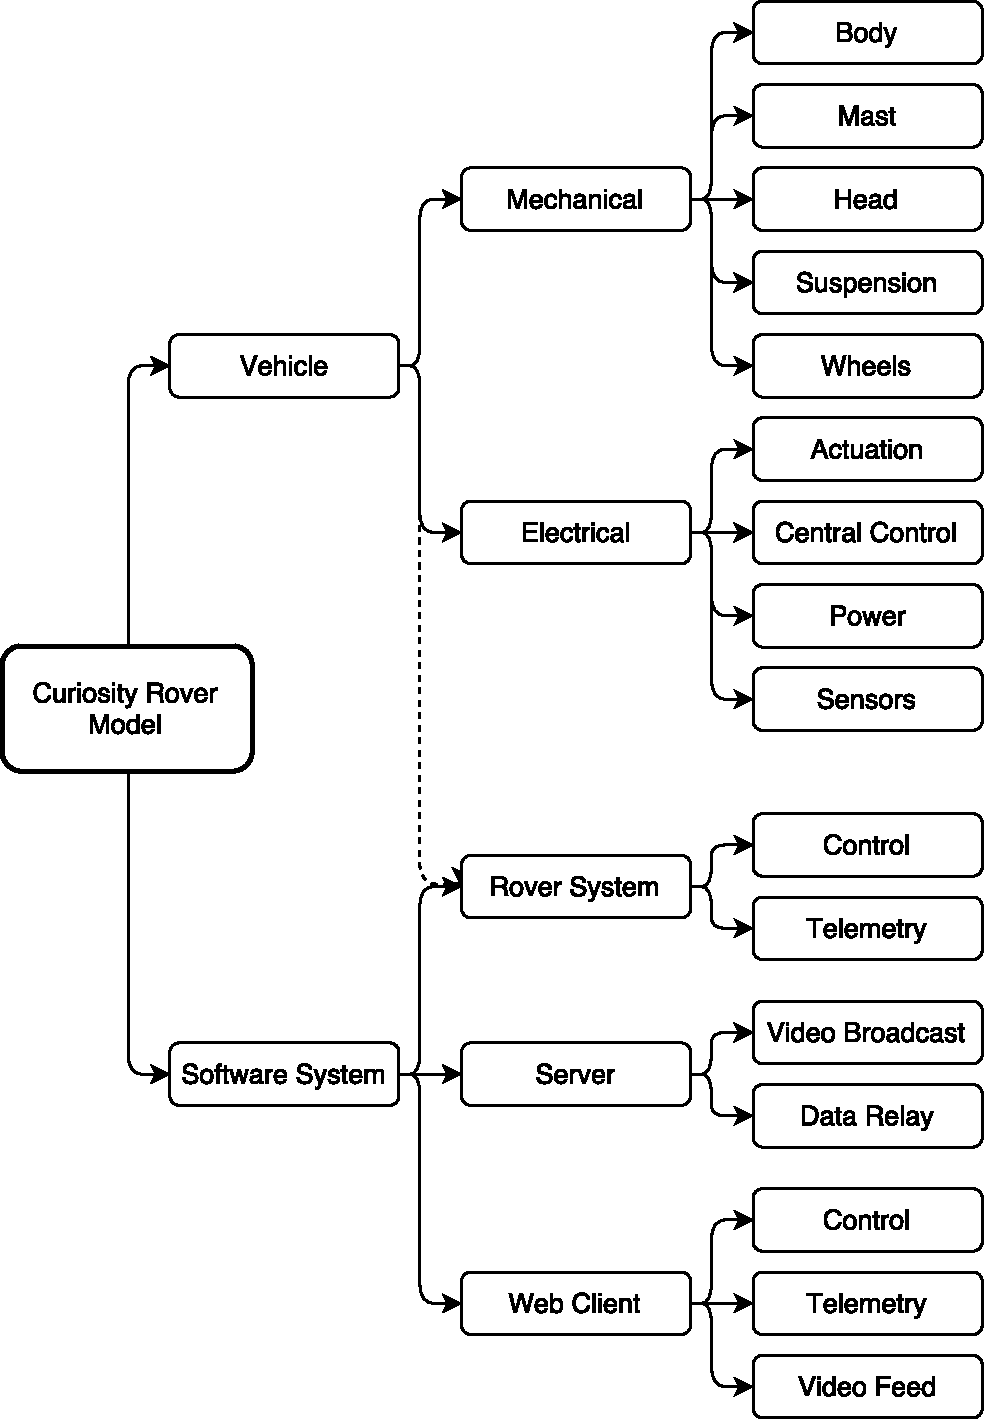
\includegraphics[width=0.6\textwidth]{figures/specs-functionalBreakdown}
      \caption[High-level breakdown of functional entities of the project]{High-level breakdown of functional entities of the project}
      \label{fig:specs-functionalBreakdown}
    \end{figure}
    
    \subsubsection{Rover Equivalence and Terminology}
    \label{subsubsec:rover-equivalence}
      Following the educational theme of the project, much of the terminology used on \textit{Curiosity} was borrowed for use in subsystems and components on the model, in both mechanical and software aspects.
      
      ![Fill out]
    
    
  \subsection{Technical Specifications}
    The technical specifications were derived from the client requirements and the functional analysis, with knowledge of the systems and subsystems on \textit{Curiosity} (taken from review of literature as covered in Chapter~\ref{chap:lit-review}. The specifications further compartmentalised the vehicle and software systems as evident in the structure of them in the lists that follow. These technical specifications served as the baseline requirements for the final design.
    
    \subsubsection{Vehicle Specifications}
    \label{subsec:probDef-vehicleSpecifications}
      \begin{itemize}
        \item \textbf{Mechanical}
        \begin{RM}
          \item General Specifications:
          \begin{RM}
            \item Be as dimensionally accurate as possible to the Curiosity rover on Mars
            \item\label{li:probDef-spec-mechanical-realism} Exhibit a satisfactory level of realism and external aesthetic accuracy
          \end{RM}
          \item Body:
          \begin{RM}
            \item Box shaped
            \item Allow mounting of the mast and differential on the top surface
            \item Allow mounting of the suspension system on either side
            \item Allow mounting of additional sensors
            \item Allow mounting of additional detail such as side panels and other mockup objects
            \item Allow mounting of electrical internals
            \item Provide protection/coverage of electrical internals from the external environment
          \end{RM}
          \item Mast:
          \begin{RM}
            \item Provide mount point for the head module
            \item Facilitate full rotation about the $z$-axis (camera panning/yaw axis)
            \item Facilitate at least $120^\circ$ degrees rotation about the $y$-axis (camera pitching axis)
            \item Be structurally secure providing robustness against lateral forces on the mounted head module
          \end{RM}
          \item Head:
          \begin{RM}
            \item Be mounted onto the mast module
            \item Provide mount point for a sensor
            \item Allow mounting of a camera module
          \end{RM}
          \item Suspension:
          \begin{RM}
            \item Ensure body stability
            \item Maintain stability despite uneven terrain. This includes terrain which might require asymmetrical articulation of the system (a rock underneath one side of the rover and flat terrain underneath the other)
          \end{RM}
          \item Wheels and Hubs/Pivots:
          \begin{RM}
            \item Match the shape and proportion of the wheels on \textit{Curiosity}
            \item Provide traction required for an analogue Martian terrain
            \item Have steering capabilities which would amount to arc pattern traversal as well as rotation of the rover around a central fixed point
          \end{RM}
        \end{RM}
        
        \item \textbf{Electrical}
        \begin{RE}
          \item Actuation:
          \begin{RE}
            \item Provide continuous rotational actuation for driving. The actuation speed should be controllable and must be of high enough torque to satisfy traversal specifications
            \item Provide sufficient magnitude rotational actuation for turning of the wheels for steering. The rotational position should be controllable and must be of high enough torque to facilitate turning of the wheels in-place
            \item Provide required magnitude rotational actuation for panning and pitching of the head/mast module. Both axes must allow positional control
          \end{RE}
          \item Central Control:
          \begin{RE}
            \item Host onboard software system for control of hardware
            \item Facilitate wireless communications with the server
            \item Interface with actuation and sensory input hardware
            \item Have performance capabilities sufficient for processing and streaming of video data from the head module
          \end{RE}
          \item Power:
          \begin{RE}
            \item Provide power for the central control hardware as well as actuation and sensor hardware components
            \item Power supply unit must fit inside or on the body module
            \item Have the ability to be turned switched off or on
            \item Allow convenient removal of source
            \item Allow easy access to charging ports
            \item Provide a means of indication of voltage for telemetry and low-battery warnings
          \end{RE}
          \item Sensors:
          \begin{RE}
            \item\label{li:probDef-spec-sensors-immediateObstacleData} Provide immediate environment data required to implement elementary obstacle detection and avoidance
            \item Be mounted in locations similar to those on \textit{Curiosity}
            \item Be compatible with the central control module in terms of data interface
          \end{RE}
          \item Camera:
          \begin{RE}
            \item Facilitate a monoscopic video feed
            \item Be mountable inside the head module
            \item Be compatible with the central control module in terms of data interface
          \end{RE}
      \end{RE}
    \end{itemize}
      
    \subsubsection{Software System Specifications}
      \begin{itemize}
        \item \textbf{Rover Embedded Software}
        \begin{RS}
          \item General Specifications:
          \begin{RS}
            \item Allow connection of a remote client for telemetry and control as well as another for video streaming
            \item Be robust against hardware errors and intermittent communication so as to maintain operation in these circumstances
          \end{RS}
          \item Control:
          \begin{RS}
            \item Provide a programmatic means to peripheral hardware access
            \item Translate control input commands into hardware output signals for control of peripheral hardware components
            \item Declare/define and execute programmatic sequences facilitating procedures such as system booting, communication initialisations, hardware initializations, self diagnosis and emergency modes
          \end{RS}
          \item Telemetry:
          \begin{RS}
            \item Emit system telemetry to the connected client consisting of system, process and hardware state as well as sequence execution notifications
          \end{RS}
          \item Video Stream:
          \begin{RS}
            \item Provide a stream of the video data to the connected client
            \item Provide video resolution on or above VGA (640$\times$480) resolution
          \end{RS}
        \end{RS}
        
        \item \textbf{Server}
        \begin{RS}[resume]
          \item General Requirements:
          \begin{RS}
            \item Manage communication with the rover system
            \item Manage communication with the connected web clients
            \item Serve web application to the connected web clients
            \item Manage roles of the connected web clients with respect to their level of access and ability to control the rover
          \end{RS}
          \item Video Broadcast:
          \begin{RS}
            \item Connect to and accept video data from the rover video stream
            \item Broadcast video stream to a scalable number of connected user clients
            \item Be robust against communication intermittency in terms of connection with the rover system
          \end{RS}
          \item Data Relay:
          \begin{RS}
            \item Relay control input commands from a controlling web client to the rover
            \item Provide a means of simulating long-distance communication 
            \item Relay telemetry data from the rover system to the connected web clients
            \item Relay state information of the rover system and server system to the connected web clients
          \end{RS}
        \end{RS}
          
        \item \textbf{Client}
        \begin{RS}[resume]
          \item Control:
          \begin{RS}
            \item Provide two means of control of the rover, if access is granted:
            \begin{enumerate}
              \item RoSE-style command sequence input, allowing composition of a sequence of commands and playback of such commands
              \item Interactive joystick/button interface
            \end{enumerate}
          \end{RS}
          \item Telemetry:
          \begin{RS}
            \item Accept and display telemetry received from the rover via the server and from the server itself
          \end{RS}
          \item Video Feed:
          \begin{RS}
            \item Accept and display video feed received from the broadcast
          \end{RS}
        \end{RS}
      \end{itemize}